\documentclass[a4paper,10pt]{article}

\usepackage[utf8]{inputenc}
\usepackage{natbib}
\usepackage[vmargin=2cm]{geometry}

\setlength{\bibsep}{1pt}
\usepackage{graphicx}
\graphicspath{{Figures/}}

\renewcommand{\bibfont}{\small}


%\title{Project report - Object Recognition and Computer vision}
\title{%
	\huge{Assembling LEGO set with augmented reality instructions}\\ \bigbreak
  	\Large{Project report}\\ 
  	\Large{Object Recognition and Computer vision - MVA}
}
\author{Othman Sbai, Pierre-Alain Langlois}
\date\today

\pdfinfo{%
  /Title    (Project proposal - Computer vision - Sbai & Langlois)
  /Author   (Othman Sbai, Pierre-Alain Langlois)
  /Creator  (Pierre-Alain Langlois, Othman Sbai)
  /Subject  (Augmented reality - tracking)
  /Keywords (augmented reality neural network ponts)
}

\begin{document}

\maketitle

\section{Introduction}
The advent of augmented reality devices such as Microsoft Hololens, Sony SmartEyeglass or Google Glass and others have made possible many interesting applications that augment the visual experience of the user with 3D holograms that are blended on his reality. Applications range from interior decoration and design, gaming but also increasing productivity in businesses by enhancing the real world and giving birth to broader imagination.

Among the applications of this new promising technology still in development is providing instructions for people to help them accomplish tasks either with human supervision or with annotating reality. In fact, as presented in \cite{alayrac_unsupervised_2015}, we can extract from the tutorial videos available online instructions for performing many tasks such as changing car tires, assemble furniture and also performing Cardiopulmonary rescucitation. These instructions can be efficiently provided to user with a 3D augmented reality device in the form of holograms and world annotations that are much comprehensible than paper instructions. An example of this world annotation is illustrated in the following figure~\ref{AnnotatingTheWorld}.

\begin{figure}
    \centering
    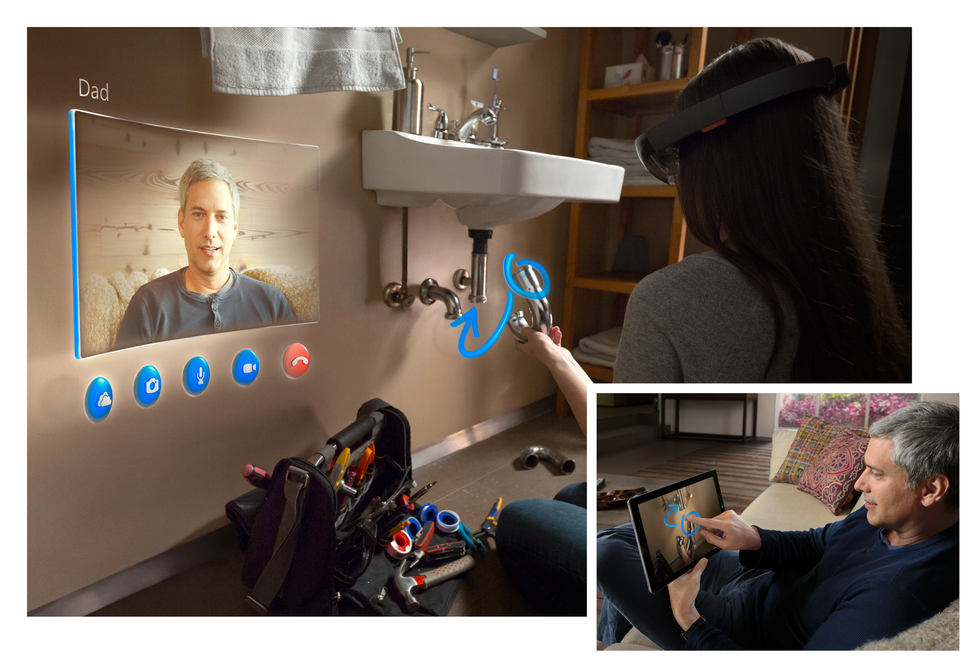
\includegraphics[width=0.75\textwidth]{Annotating_world_hololens}
    \caption{Annotating the world with Microsoft Hololens}
    \label{AnnotatingTheWorld}
\end{figure}

\newpage

We have chosen the topic : \emph{A.3 Instructions for assembling simple lego objects}.
\smallbreak
The advent of augmented reality tools such as Microsoft Hololens have made possible many interesting 
applications that augment the visual experience of the user providing relevant informations and 
distractions. Across the web, one can find lots of tutorial videos for performing a certain task be it 
assemble a furniture, prepare a meal, change tire in addition to DIY videos. These explanations can 
really be enhanced through augmented reality technology by overlaying instructions in the view of Hololens 
for example in order to adapt the tutorial to the real world’s configuration. 
\smallbreak

We propose to tackle the problem of providing instructions for assembling simple LEGO set. This simple 
game-related problem is a good start in manipulating and recognizing 3D objects from a head-mounted camera. 
Our goal is to create an assistant that is able to recognize the state of the LEGO mounting problem and 
suggest the next step by blending virtual movement on the reality perceived by the player thanks to 
Hololens.

\smallbreak

We will first implement a system that allows to recognize and locate the pieces in the frame in real time~\cite{redmon_you_2015}. 
This system will provide simple informations to help the user assembling the pieces.

If the system works well enough, we will try to add the pose estimation in the process in order to give 
more precise informations about the pieces orientation~\cite{wohlhart_learning_2015}.

\smallbreak
Some researchers already worked on the problem of LEGO brick identification and retrieval in realtime from 
2D images\cite{botha_realtime_2009}. In our case, we will generate data directly from the hololens (both 
RGB and geometrical data), since we have only a few lego pieces to recognize. If needed, we will also use 
data augmentation techniques. 
 
\section{Plan of work}

\begin{itemize}
 \item GOAL: Implement an interactive assistant that helps solving/assembling a LEGO set. Providing relevant statistics to evaluate the performance of the method.
 \item We assume the knowledge of the set of sequences required for the assembly, this can be either 
 supplied by LEGO from the manual, or can be deduced from tutorial videos, as was done in the paper 
 \cite{alayrac_unsupervised_2015}.
 \item From a head mounted camera, recognize LEGO part to be moved and its destination and display a 
 hint of the movement overlaid on the hololens.
 \item If the previous work is good enough, we will try to add support for pose estimation and more 
 advanced instructions.

\end{itemize}


\section{Operational organization}

\subsection{Group members}

\begin{itemize}
 \item Othman Sbai (MVA \& École des Ponts ParisTech)
 \item Pierre-Alain Langlois (MVA \& École des Ponts ParisTech)
\end{itemize}


\subsection{Plans for work sharing}

%Object detection & pose estimation
Pierre-Alain will be focused on the work regarding the object detection (including segmentation) and the 
pose estimation task.
%Tracking & implementation on Hololens
Othman will be focused on the tracking constraints, and the implementation and experiments on the hololens 
device. Both of us will also perform testing on each other implementations in order to make the produced 
code more robust.


\bibliographystyle{plain}
\bibliography{biblio}


\end{document}
